\chapter{Eksperimen \textit{In-place Resource Resize} untuk \textit{pods Kubernetes}}
\label{appendix:eksperimen-in-place-resource-resize}

\textit{In-place Resource Resize} adalah fitur untuk mengubah ukuran sumber daya CPU dan memori yang dialokasikan untuk kontainer pada pod yang sedang berjalan tanpa harus me-\textit{restart} pod atau kontainernya. Sebuah \textit{node} Kubernetes mengalokasikan sumber daya untuk sebuah pod berdasarkan permintaannya, dan membatasi penggunaan sumber daya pod berdasarkan batasan yang ditentukan dalam kontainer-kontainer pod tersebut. Fitur ini baru hadir pada versi Kubernetes 1.27.0, dan, pada saat tugas akhir ini dikerjakan, masih dalam tahap \textit{alpha testing} dan pengembangan. Dokumentasi resmi dipublikasikan pada 30 Maret 2023 7:59 PM PST. Sedangkan, untuk publikasi \textit{alpha testing} sudah dilakukan semenjak 13 Mei 2023.

\begin{enumerate}
    \item \textbf{Persiapan Kakas}

        Terdapat beberapa kakas yang harus disiapkan terlebih dahulu sebelum melaksanakan eksperimen ini, diantaranya sebagai berikut.

        \begin{enumerate}
            \item Kubernetes Client v1.27.1-eks-2f008fe
            \item Minikube 1.30.0 yang berisikan Kubernetes v1.27.0-rc0
        \end{enumerate}

    \item \textbf{Pengerjaan Eksperimen}
        
        Dalam melakukan eksperimen ini, dilakukan beberapa tahap sebagai berikut.

        \begin{enumerate}
            \item Memastikan versi Kubernetes yang digunakan adalah versi 1.27.0 atau lebih baru pada \textit{client} dan \textit{server}.
            
            Pada saat pengerjaan implementasi, Kubernetes lokal yang dipakai adalah \textit{Docker Desktop Kubernetes} yang membatasi versi Kubernetes pada versi 1.25.9. Sehingga, dilakukan pengubahan server dengan menggunakan Minikube versi 1.30.0. Namun, versi maksimal yang bisa dipakai oleh Minikube 1.30.0 adalah Kubernetes versi 1.27.0-rc0, versi 1.27 yang paling pertama atau \textit{release candidate 0}. Untuk mengecek bisa dilihat pada \url{https://github.com/kubernetes/minikube/releases/tag/v1.30.0}. Dicoba juga untuk dipaksa menggunakan versi 1.27.1 maupun 1.27.3, namun hal tersebut gagal untuk dilakukan. Sehingga, untuk eksperimen ini, digunakan Kubernetes versi 1.27.0-rc0 melalui Minikube.

            \item Membuat \textit{deployment} yang akan digunakan untuk eksperimen.
            
            Konfigurasi \textit{deployment} berubah, karena untuk menggunakan fitur ini, tidak bisa membuat \textit{pods} dengan menggunakan tipe \textit{deployment} melainkan harus langsung membuat dengan tipe \textit{pod}. Terdapat juga beberapa konfigurasi baru yang perlu diatur, lihat gambar \ref{fig:appendix1-kube-config}.

            \item Mengeksekusi perintah untuk melakukan \textit{in-place resource resize}.
            
            Hal ini bisa dilakukan dengan mengeksekusi perintah \textit{patch pod}. Perintah ini bisa dilihat pada dokumentasi: \url{https://kubernetes.io/docs/tasks/configure-pod-container/resize-container-resources/}.

            Saat hal ini dijalankan terdapat pesan eror yang mengatakan bahwa fitur \textit{patch} tersebut hanya bisa dilakukan selain resource, lihat gambar \ref{fig:appendix1-eksperimen-gagal}. Padahal, inisiasi eksperimen sudah disesuaikan dengan \textit{requirement} yang disebutkan pada dokumentasi, lihat gambar \ref{fig:appendix1-kube-doc}.

            \begin{figure}[h]
                \centering
                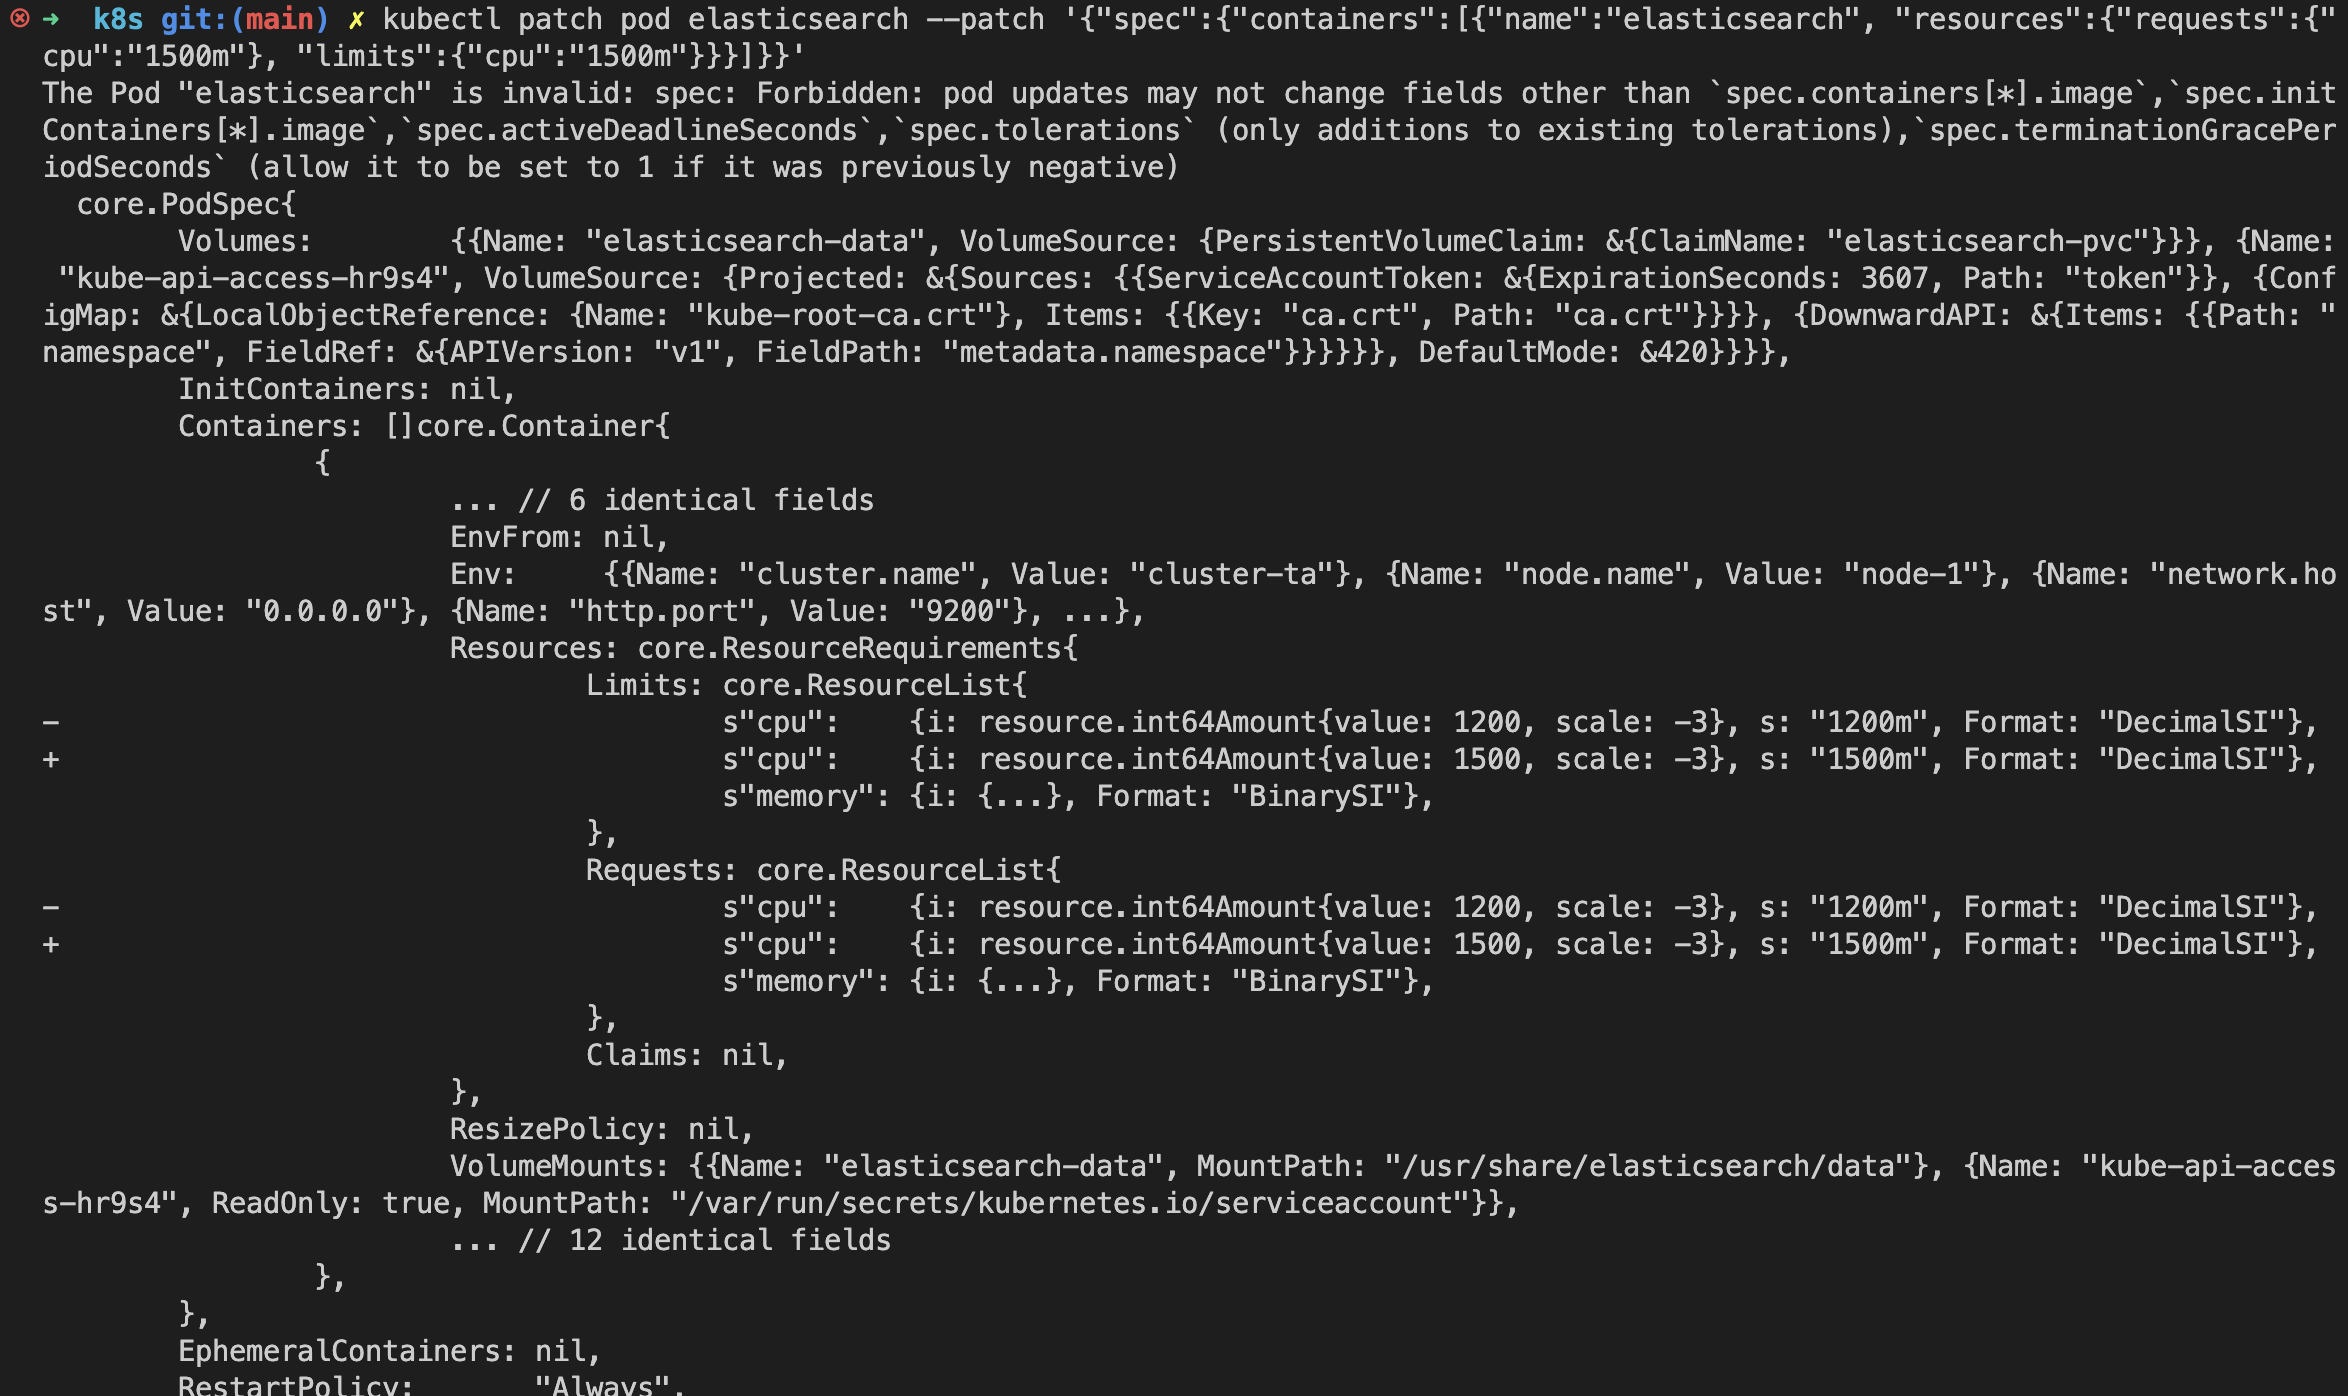
\includegraphics[width=1.1\textwidth]{appendix/eksperimen-gagal.png}
                \caption{Pesan Error saat Melakukan \textit{Patch} pada \textit{Pods}}
                \label{fig:appendix1-eksperimen-gagal}
            \end{figure}

            \begin{figure}[h]
                \centering
                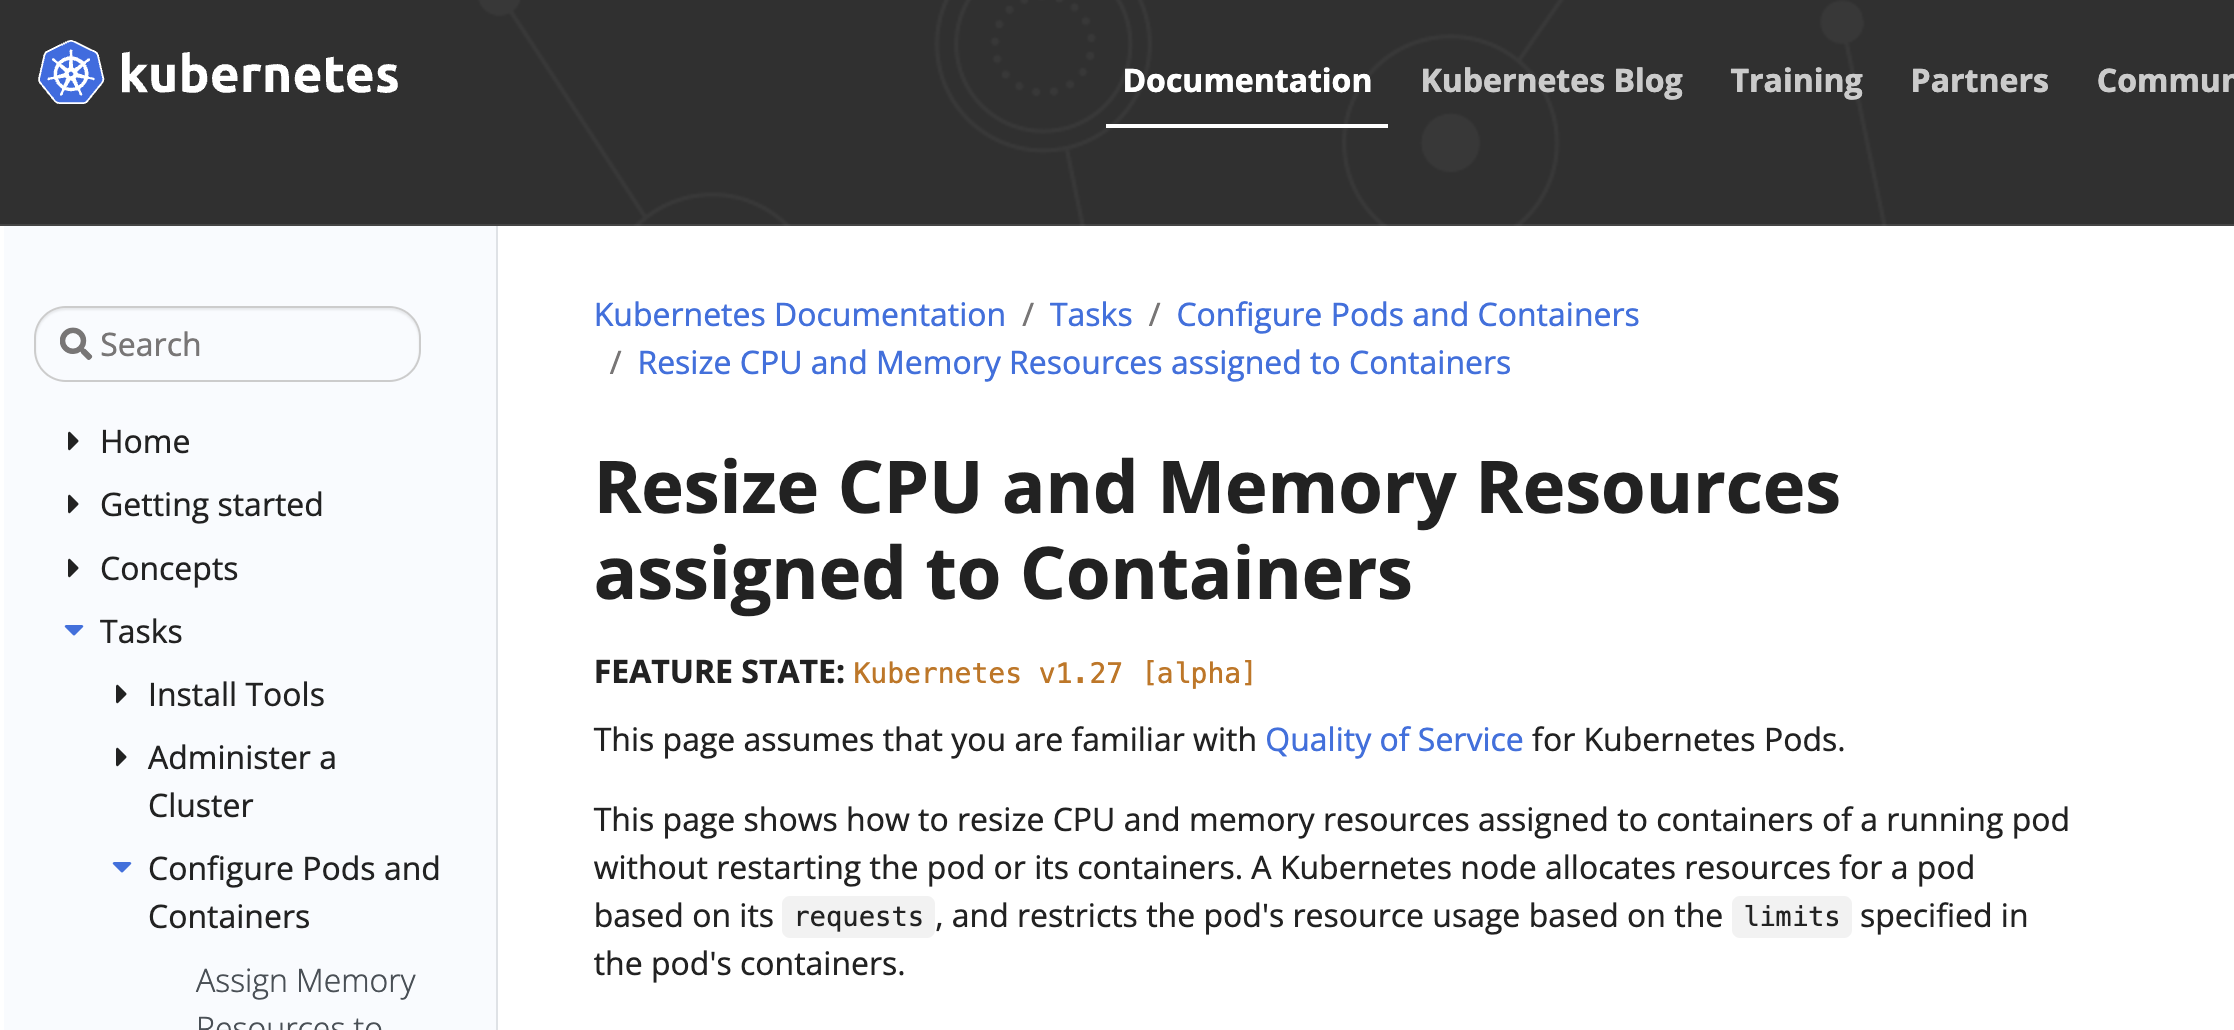
\includegraphics[width=1.1\textwidth]{appendix/kubernetes-docs-resize.png}
                \caption{Dokumentasi Kubernetes: \textit{In-place Resource Resize}}
                \label{fig:appendix1-kube-doc}
            \end{figure}

            \item Mengecek detail informasi \textit{pods}
            
            Seharusnya, ketika mengecek detail informasi \textit{pods} akan terlihat bahwa resource yang digunakan sudah berubah dan terdapat informasi-informasi baru yang hanya muncul pada versi terbaru Kubernetes, contoh bisa dilihat pada gambar \ref{fig:appendix1-info-terbaru}. Namun, hal ini tidak terjadi. Resource yang digunakan masih sama dengan sebelumnya. Dan hasil detail informasi sebuah \textit{pods} tidak memperlihatkan detail informasi terbaru yang sesuai dengan contoh pada dokumentasi.

            \begin{figure}[h]
                \centering
                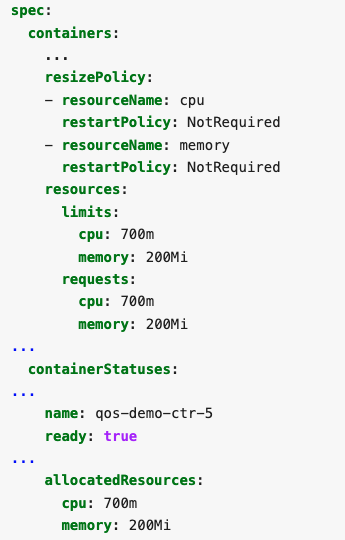
\includegraphics[width=0.6\textwidth]{appendix/cth-info-terbaru.png}
                \caption{Dokumentasi Kubernetes: Detail Informasi \textit{Pods} Tambahan pada Versi Terbaru}
                \label{fig:appendix1-info-terbaru}
            \end{figure}
        \end{enumerate}

    \item \textbf{Hasil Eksperimen}
    
        Berdasarkan hasil eksperimen tersebut, dapat disimpulkan bahwa.

        \begin{enumerate}
            \item Fitur \textit{in-place resource resize} belum bisa digunakan pada Kubernetes versi 1.27.0-rc0.
            \item Karena keterbatasan saat melakukan eksperimen, tidak dicoba dengan versi 1.27.3 atau diatasnya karena kubernetes lokal dengan Minikube 1.30 (terbaru pada saat ini ditulis) maupun Kubernetes Docker Desktop belum bisa menggunakan versi tersebut, lihat gambar \ref{fig:appendix1-minikube} pada bagian \textit{Version Upgrades}.
            \item Melakukan \textit{resource resize} tanpa melakukan \textit{restart} bisa dilakukan pada masa yang akan datang, hanya perlu menunggu sampai fitur ini stabil.
            \item Eksperimen ini bisa dicoba lagi pada masa yang akan datang. Mengingat tools kubernetes lokal masih belum bisa menggunakan versi \textit{alpha} terbaru.
        \end{enumerate}

        \begin{figure}[h]
            \centering
            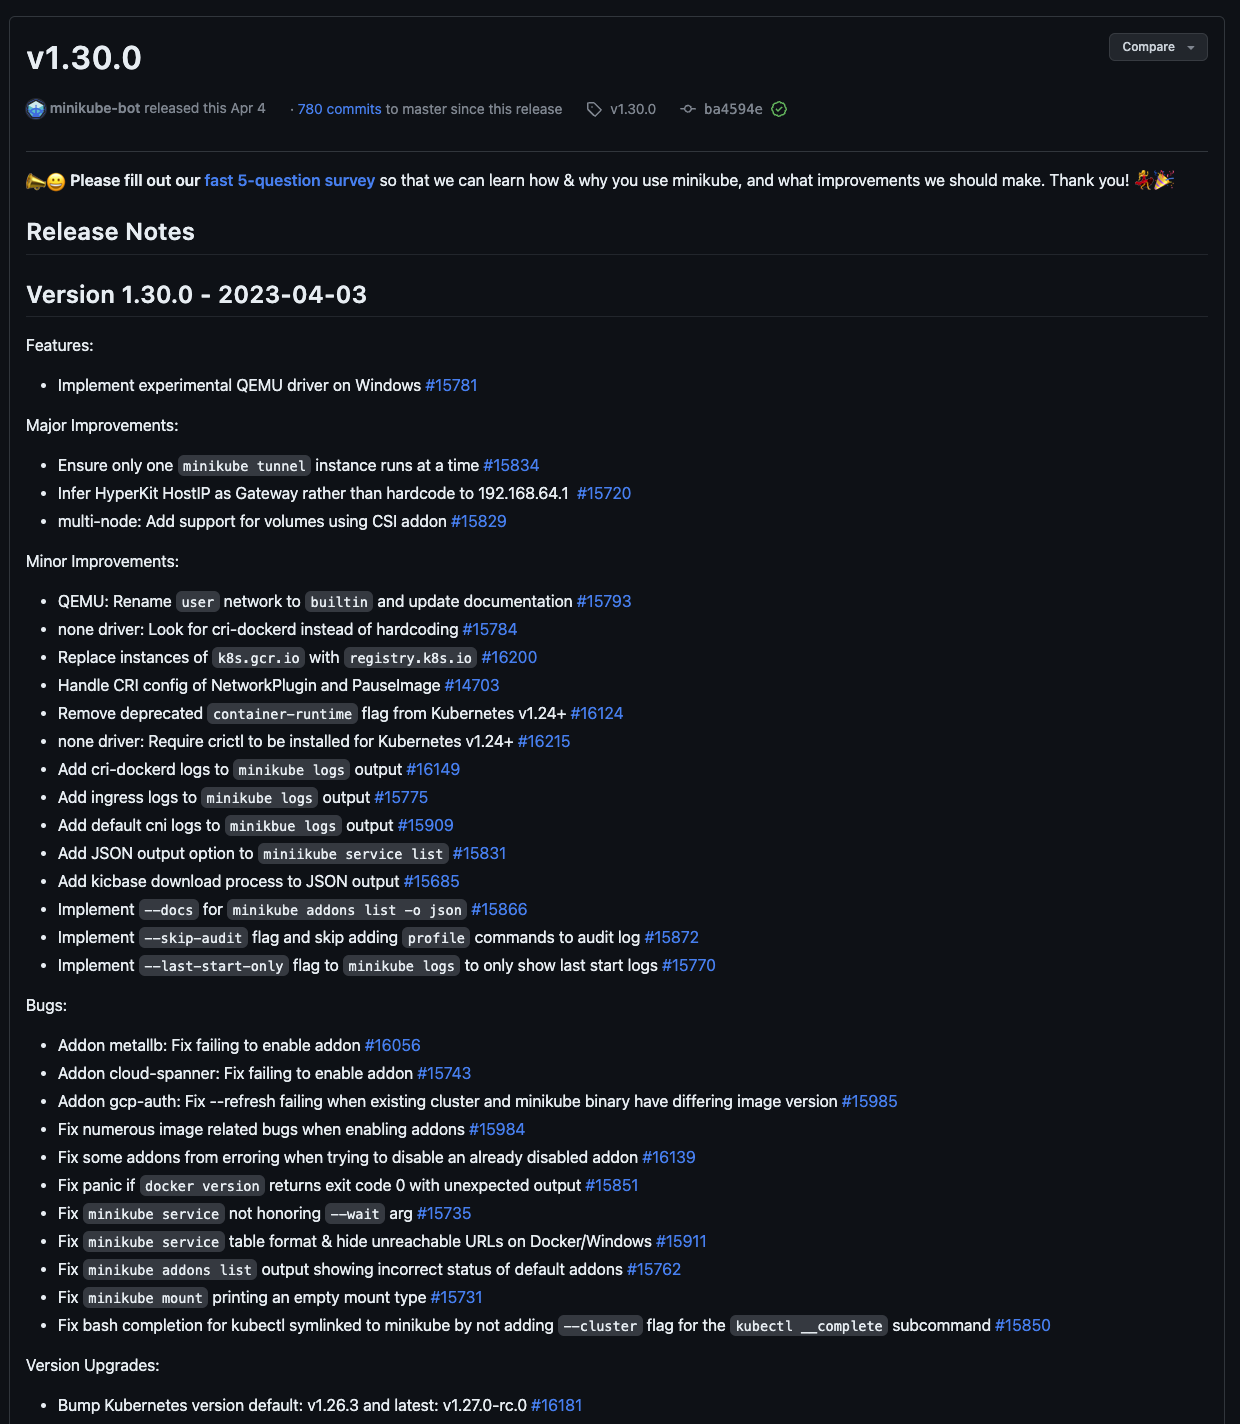
\includegraphics[width=1\textwidth]{appendix/minikube-130.png}
            \caption{Informasi \textit{Update} Minikube 1.30.0}
            \label{fig:appendix1-minikube}
        \end{figure}
\end{enumerate}

\begin{figure}[h]
    \centering
    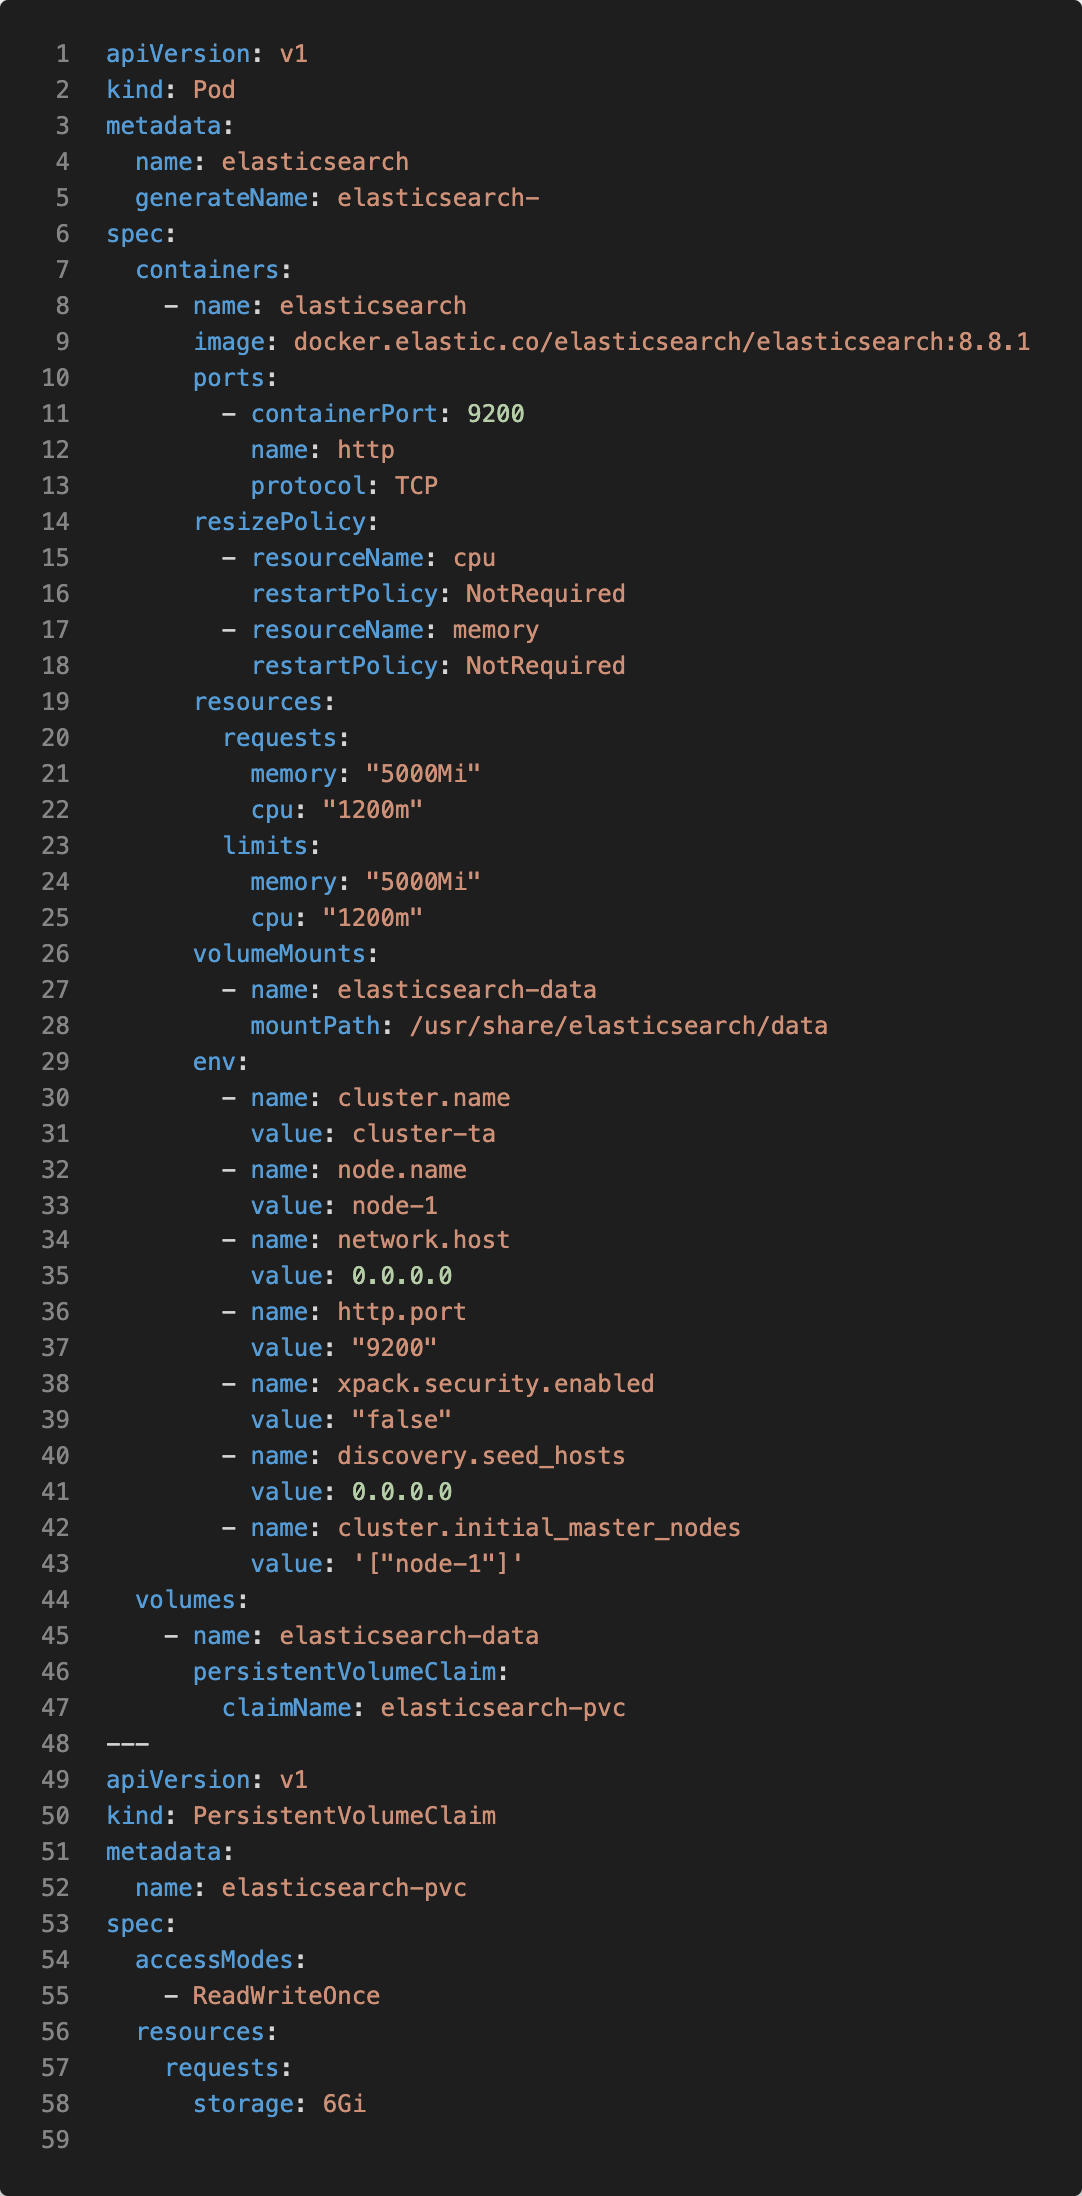
\includegraphics[width=0.75\textwidth]{appendix/konfigurasi-kube.png}
    \caption{Konfigurasi \textit{Pods} untuk Eksperimen}
    \label{fig:appendix1-kube-config}
\end{figure}